\chapter{Sampling on Hadoop} % (fold)
\label{cha:sample}

In this chapter we present one method for data sampling on hadoop that is basead
in a random algorithm.

\section{Motivation for sampling}

One relevant aspect in Big Data environment is the vast amount of data,
that is the main barrier to find a good job configuration job. The bacteriological
algorithm is an option to create new configurations, but these configurations
must be tested in order to select which is the best for the job at the a given
moment. Moreover, the dynamism of the computing nodes, joining and leaving, big
cluster setups at any time and data volatility, may spoil performance depending
on the configurations setup. 

Therefore, caused for these dynamisms described the job configuration needs to be
reviewed constantly. This review process consist in to choose a new configuration
and to test it in order to analyse the performance. But the test step cannot be
done on the entire data.

{\it So, how must we test the job configurations generated by BA?} One possible
answer is to run the job on data sampling, because the sampling in a database is
a essential step to improve the response time, moreover run the job on all data
stored would spend much time and also would be impracticable due larger number
of intermediate configurations generated by the algorithm.

\section{Challenge for data sampling in Big Data environments}

On Big Data environment there are several aspects involving distributed computing
and storage. For data sampling the aspects involving storage distributed are more
relevant. In this context, without doubt, the data volume is the main issue because
the data sampling must be done distributed too, otherwise one machine couldn't bear
all data storage in the cluster then make the data sampling, e.g. suppose that
one cluster storage 100 terabytes and we want data sampling of 20 percent, then
each node must do local sampling and store it locally, so the resultant sample will
be 20 terabytes which one conventional machines doesn't have this storage capacity.

So the resultant data sample must be storage distributed in the cluster, because
even being a sample the result can be big and a single machine couldn't bear too.
After the sampling obtained, jobs can run on the sampling, avoiding to run on 100
terabytes and run just 20 terabytes as the example.

%So the sampling must be done distributed and it must be done without intrusion
%in the Hadoop, because any change done inside of the framework can propagate collateral
%effects due its complexity. Further more to run test regression is a very costly
%activity~\cite{hadoopUnit} and to create unit test cases for the new changes spend
%much time.

The Hadoop has the structure for distributed storage, so one way to obtain data
sample data is to utilize its benefits, i.e. taking into consideration that the
data already are distributed storage, so we can build one MapReduce program to
sample data and we will be benefiting of its advantages as framework to distributed
computing.

One of the most used data sample techniques is {\bf Random Sampling} that consists
in selecting a pre-determined amount of data randomly~\cite{randomsampling}.
In the literature there are several others techniques such as {\bf Stratified Random Sampling},
which splits data in strata where each element has the same chance of being selected
~\cite{randomsampling}. Another thechnique is {\bf Systematic Sampling} that has
one number {\it k} which is chosen randomly or chosen with some criteria, then
randomly one element is chosen of the population and from this element till the
next k-esimo elements in sequence are selected to sample~\cite{systematicsampling}.

In the context of big data there are some implementations of data sample. One example
is the {\bf MonetDB} which is column-oriented database management system and was
designed to hold data in main-memory and processes large-scale data distributed~\cite{monetDB},
this database support data sample and use the {\it Algorithm A} that is based in
random sample method~\cite{monetDB:sampling}.

The algorithm A select {\it n} records from a file containing {\it N} records where
$0\le{\it n}\le{\it N}$. For each record that will be inserted in the sample,
it chooses randomly one number {\it V} that is uniformly distributed between 0 and 1.
Based in {\it V, n} and {\it N} is calculated the number {\it s}, from {\it s}
is created the records set called {\it S}, this set will contain the {\it (s + 1)}st
records in the file, then one record is chosen from {\it S} and put in the sample.
The records present in {\it S} are skipped in the next interaction~\cite{vitter:1984}.

Another database management system that performs data sampling based on random methods
the {\bf Hive} a data warehouse system for Hadoop. It samples in
row or block size level. The row level consists in choosing randomly the rows
according with the colunm name. If the column name is not defined, then the entire row
is selected. With the colunm name defined the choice can be done using the
{\bf Bucketized Table} in which the sample is done only on the buckets that contains
the specified column~\cite{hiveSample}. The block size sample is also done ramdomly
and consist in selecting the blocks that match with the specified block size.

Those sample methods on Hive are based in random sample and handle structured data.
The Hive principle is just store the Hadoop data as a data warehouse and facilitate
queries submitted by users. Moreover, the clustering by bucket and block size concept
requires a prior structuring of data, so in the Hive several information about the
data are previously known.

In Hadoop, data are stored unstructured and this characteristic is the
biggest challange to develop data sampling. According to~\cite{vitter:1985, cloudera, greg, wikipedia:ReservoirSampling}
the challange with unstructured data stream can be addressed with {\bf Reservoir Sampling}:
"{\it Say you have a stream of items of large and unknown length that we can only
iterate over once. Create an algorithm that randomly chooses an item from this
stream such that each item is equally likely to be selected.}"

The Reservoir Sampling is part of the randomized algorithm family and consists in
choosing randomly {\it k} elements from a list {\it L} containing {\it N} items.
The length N is either unknown or large enough to fit in memory. See algorithm~\ref{alg:sample}.

\begin{algorithm}
		\caption{Algorithm for Reservoir Sampling \label{alg:sample}}

        \SetKwInOut{Input}{Input}
        \SetKwInOut{Output}{Output}
		\Input{$k$ size of sample}
		\Input{$stream$ data stream with indefided length}
        \Output{$arraySample$[$k$]}

		\For{$i = 1 \to k$} {
			$arraySample[i] \leftarrow stream[i]$
		}

		$nextElement \leftarrow k$

		\While{$stream$ != $EOF$} {
			$nextElement \leftarrow nextElement + 1$

            $probability \leftarrow k/nextElement$

			$chance \leftarrow Random(0,1)$

			\If {$chance < probability$}
			{
                $pos \leftarrow Random(1,k)$

				$arraySample[pos] \leftarrow stream[nextElement]$
			}
		}

        \Return{$arraySample$}
\end{algorithm}

The goal is to build a reservior smaller than the memory. So
it receive as parameter the number {\it k} that is the resultant sampling length
and {\it stream} of data that constantly receive new data. Initially the resultant
sampling is assigned with the first {\it k elements}, so the algorithm
aim to calculated the probability of the next element, e.g. {\it k+1}, to be inserted
to the sample, which is {\it P(k+1) = k/(k+1)}, after one random number({\it chance})
between 0 and 1 is chosen, if {\it chance $<$ P(k+1)}, then the next element is putted
in random position in the resultant sample.

However, choosing the number {\it k} is a hard task, because the resultant sample must
be representative and fit in memory. To solve that problem Vitter~\cite{vitter:1985}
suggests that the reservoir be stored on secundary storage(hard disk). But this
approach may be implactible on the Hadoop context, because the secundary storage
is HDFS and the time of retrieving the reservoir and update is very large, because
of the override among contact namenode, it look up the reservoir in the cluster
and make it available.

\section{One method for data sampling on Hadoop}

We propose the follow algorithm based on the MapReduce paradigm to generate data
samples on Hadoop. It follows the random algorithm family which has been used largely
in database and big data environment.

First of all, we will present the behavior of the algorithm on map and reduce process
using the Figure~\ref{fig:sampleProcess}, Initially the program receives tree files:
file1, file2 and file3. There are two mappers to classify each line of the files
and generate the output \tuple{lineNumer, content}. Then, the shuffle step
aggregates each content of the same key \tuple{lineNumer, \{content1, content2, ..., contentN\} }.
The only reducer receives the shuffle output and, for each content of the same key,
chooses one random number. If it is less than sample threshold then chooses this
content, otherwise discards it.
\\
\\
\\
\\
\begin{figure}[htbp]
	\centering
	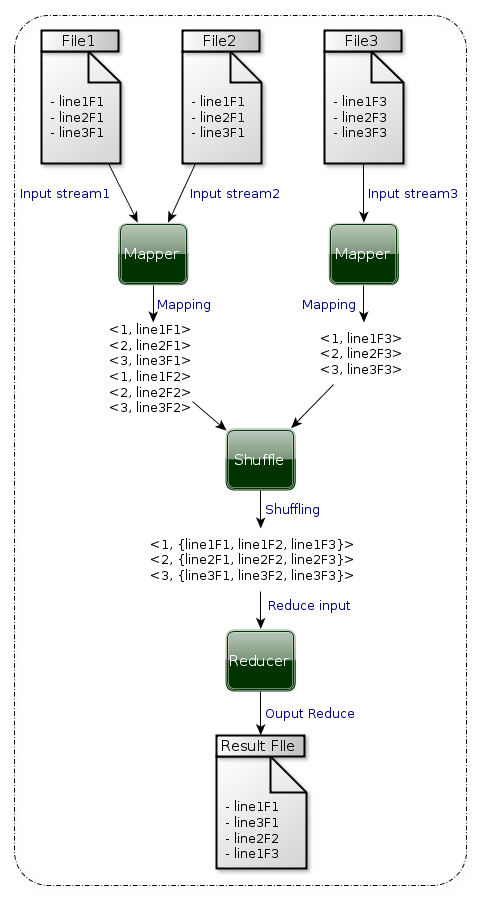
\includegraphics[width=210px,height=400px]{img/sampleProcess.png}
	\caption{Map and Reduce random sample process}\label{fig:sampleProcess}
\end{figure}
\\

The map function is described by algorithm~\ref{alg:map}. Before presenting the
algorithm, some previous definitions are necessary. Let us denote {\it F} the files
set storage on the cluster, {\it f} one file belonging {\it F}, {\it l} current
line of {\it f} and {\it o} the order of the {\it L} in {\it F}.

\begin{algorithm}
		\caption{Map function for data sample \label{alg:map}}

        \SetKwInOut{Input}{Input}
        \SetKwInOut{Output}{Output}
		\Input{$F$ file set in the cluster}
        \Output{$map<Integer, String>$ 	resultant list of key-value}

		$map \leftarrow  \{\}$

		\For{\textbf{each} $f \in F$} {

			$l \leftarrow f.getNextLine()$

	    	$o \leftarrow l.getOrder()$ 

			$map.put$($o$, $l$)

		}

        \Return{$map$}
\end{algorithm}


The map function consists in classify each {\it L} in the {\it F} with
it respective order {\it o}. Then intermediate key-value pair \tuple{o, l}
are emitted. Next, each pair is added to a map structure that is the output of
the map function. After the shuffle phase aggregates values sharing the same key.
This aggregated values are the input for reduce function.

\begin{algorithm}
		\caption{Reduce function for data sample \label{alg:reduce}}

        \SetKwInOut{Input}{Input}
        \SetKwInOut{Output}{Output}
		\Input{$mapList<key, values>$ list of key-values aggregated by shuffle phase}
        \Output{$list$ of selected values}

		\For{\textbf{each} $key \in mapList$} {

			\For{\textbf{each} $v \in values$} {
				$rand \leftarrow random(1, n)$

				\If{$rand \leq n$} {
					$list.add(v)$
				}

			}

		}

        \Return{$list$}
\end{algorithm}

The reduce function is in charge of the sampling and is described by algorithm~\ref{alg:reduce}.
Before presenting the algorithm, some previous definitions are necessary. Let us
denote {\it mapList} the intermediate set generated by map phase and aggregated
for the shuffle phase, it contains tuples \tuple{key, list<values>}. The {\it key}
is one key belonging the {\it mapList} and {\it values} are a set of values sharing
the same key. The {\it v} is one value belonging to {\it values} and {\it n} is
the lenght of the values sharing the same key.

First the reduce algorith iterates in each {\it key} and get the {\it values}
list. Then for each value {\it v} that sharing the same key, one random number
between the 1 and {\it n} is chosen. If the random number is less than equal
{\it n} then {\it v} is added to resultant list. 
